%\documentclass[twoside]{pwrthesis}
\documentclass[twoside]{iisthesis}
% ---
\usepackage{polski}
\usepackage[utf8]{inputenc}
\usepackage{amsmath}
\usepackage{tocloft}
\usepackage{listings}
\usepackage{algorithm}
\usepackage{algorithmic}
\usepackage{subcaption}
\usepackage{mathtools}
\usepackage{graphicx}
\usepackage[colorinlistoftodos]{todonotes}
\usepackage{url}
\usepackage{pgfplots, pgfplotstable}
\selectlanguage{polish}
% Dodane przeze mnie d
\usepackage{fancyvrb} % dla srodowiska Verbatim
\usepackage{color}
\usepackage{lscape}

\hypersetup{
    colorlinks,
    linkcolor={black!50!black},
    citecolor={black!50!black},
    urlcolor={black!80!black}
}

\definecolor{gray}{rgb}{0.4,0.4,0.4}
\definecolor{darkblue}{rgb}{0.0,0.0,0.6}
\definecolor{cyan}{rgb}{0.0,0.6,0.6}

\lstset{
  basicstyle=\ttfamily,
  columns=fullflexible,
  showstringspaces=false,
  commentstyle=\color{gray}\upshape
}

\lstdefinelanguage{XML}
{
  morestring=[b]",
  morestring=[s]{>}{<},
  morecomment=[s]{<?}{?>},
  stringstyle=\color{black},
  identifierstyle=\color{darkblue},
  keywordstyle=\color{cyan},
  morekeywords={xmlns,version,type}% list your attributes here
}

\lstset{
  language=XML,
   literate={ć}{{\'c}}1
}
\renewcommand*{\lstlistingname}{Kod źródłowy}
% definicje kolorow
\definecolor{ciemnoSzary}{rgb}{0.15,0.15,0.15}
\definecolor{szary}{rgb}{0.5,0.5,0.5}
\definecolor{jasnoSzary}{rgb}{0.2,0.2,0.2}

% Konfiguracja verbatima
\fvset{
	frame=single,
	numbers=left,
	fontsize=\footnotesize,
	numbersep=12pt,
%	framerule=.5mm,
	rulecolor=\color{ciemnoSzary},
%	fillcolor=\color{jasnoSzary},
	framesep=4pt,
	stepnumber=1,
	numberblanklines=false,
	tabsize=2,
%	formatcom=\color{szary}
}
\newcommand{\listequationsname}{Spis wzorów}
\newcommand{\equationcaption}[1]{\begin{flushright}\emph{#1}\end{flushright}}
\newcommand{\rightcaption}[1]{\begin{flushright}\emph{#1}\end{flushright}}
\newlistof{myequations}{equ}{\listequationsname}
\newcommand{\myequations}[1]{%
\addcontentsline{equ}{myequations}{\protect\numberline{\theequation}#1}\par}

\newcommand{\listofmyalgorithmsname}{Spis algorytmów}
\newlistof{myalgorithm}{algo}{\listofmyalgorithmsname}
\newcommand{\myalgorithm}[1]{%
\addcontentsline{algo}{myalgorithm}{\protect\numberline{\thealgorithm}#1}\par}


\newcommand{\listofmyfiguresname}{Spis rysunków}
\newlistof{myfigure}{figu}{\listofmyfiguresname}
\newcommand{\myfigure}[1]{%
\addcontentsline{figu}{myfigure}{\protect\numberline{\thefigure}#1}\par}

\floatname{algorithm}{Algorytm}

\newtheorem{mydef}{Definicja}



\begin{document}


\newcommand{\resultChart}[7][140]{
\def\dataS{{#2}}
	\begin{figure}[H]
	
\centering

\begin{center}
\begin{tikzpicture}
 
\begin{axis}[
ybar,
bar width=20,
legend style={at={(0.5,-0.25)},
anchor=north,legend columns=-1},
ylabel={Wartość miary},
symbolic x coords={\dataS},
xtick=data,
height=  {#1},
width=0.8\textwidth,
ymin=0, ytick={0,0.5,1},
ymax=1.5,
nodes near coords,
nodes near coords align={vertical},
]
\addplot coordinates { (\dataS,{#3}) };
\addplot coordinates {(\dataS,{#4}) };
\addplot coordinates { (\dataS,{#5}) };
\legend{Recall,Precission,F1-Score}
\end{axis}
\end{tikzpicture}
\end{center}
\caption{{#6}}
\myfigure{{#6}}
\label{{#7}}
\end{figure}
}


\pgfkeys{/pgf/number format/use comma}
\pgfkeys{/pgf/number format/.cd, set thousands separator={}}%
\nocite{*}
\title{ Wielokryterialny problem rozmieszczenia zraszaczy wodnych na zadanej powierzchni }
\titleEN{ Multicriteria water sprinklers deployment problem on a given area}
\shortTitle{SHORT TITLE}
\author{inż. Grzegorz Dziedzic}
\advisor{dr Mariusz Fraś}
\instituteLogo{logos/pwr}
\slowaKluczowe{optymalizacja wielokryterialna,\\ algorytmy genetyczne,\\zraszacze wodne}

\date{\number\the\year}

% Wstawienie abstractu pracy
	%\input {abstract}

\abstractSH{SHORT ABSTRACT}

\abstractPL{
	ABSTRACT PL
}
\abstractEN{
	ABSTRACT EN
}

\maketitle

\textpages


\graphicspath{ {img/} }
\DeclareGraphicsExtensions{.pdf,.png,.jpg}
\chapter{Wstęp}
\section{Wprowadzenie}
Odpowiednie nawodnienie ogrodu jest jedną z podstawowych czynności pielęgnacyjnych. Gdy właściciel dysponuje odpowiednim budżetem najlepszym rozwiązaniem będzie dla niego inwestycja w automatyczny system nawadniania. System taki składa się z zraszaczy wodnych, rur pomiędzy nimi oraz systemu sterowania. Takie rozwiązanie pozwala zaoszczędzić czas tracony na ręcznym podlewaniu ogrodu oraz zapewnia równomierne nawodnienie na całej ustalonej powierzchni. Jednym z głównych problemów koniecznych do rozwiązania podczas instalacji takiego systemu jest odpowiednie rozmieszczenie poszczególnych zraszaczy. Te najczęściej znajdują się pod ziemią oraz posiadają wynurzalną głowicę. Z tego powodu raz zainstalowany zraszacz najczęściej zostaje na swoim miejscu, aż do momentu wymiany całej instalacji wodnej. Biorąc to pod uwagę rozmieszczenie zraszaczy powinno być dobrze przemyślane już podczas etapu projektowania systemu nawadniania. Projektując taki system należy przyjąć jako cel nawodnienie całości wskazanego obszaru jak najmniejszym kosztem przy przestrzeganiu wskazanych przez właściciela ograniczeń.

Proces projektowania sieci zraszaczy może być żmudny oraz długotrwały, biorąc pod uwagę różnorodność sprzętu dostępnego na rynku czy chociażby nieregularność powierzchni, która ma zostać nawodniona. Z pomocą może przyjść tutaj nowoczesna technologia. Opisany powyżej problem idealnie nadaje się do rozwiązania przy pomocy dostępnych algorytmów optymalizacyjnych. Praca ta będzie skupiać się na rozwiązaniu omówionego problemu poprzez opracowanie systemu wspomagania decyzji i implementację oraz porównanie wielokryterialnych algorytmów genetycznych.

\section{Problem nawodnienia obszaru}
Jednym z podstawowych problemów z jakim spotykają się właściciele ogrodów jest instalacja odpowiedniego systemu nawadniania. Mogą to zrobić sami albo zlecić zadanie firmie zajmujacej się projektowaniem ogrodów i systemów nawadniania.
Jest kilka szczególnie ważnych elementów, na które należy zwrócić uwagę projektując taki system:\\
\begin{itemize}
	\item Odpowiedni pomiar terenu, który ma zostać nawodniony
	\item Wzięcie pod uwagę ukształtowania terenu
	\item Obliczenie potrzebnego ciśnienia wody
	\item Wybór i rozmieszczenie zraszaczy
	\item Wybór i poprowadzenie rur
	\item Umiejscowienie zaworów\\
\end{itemize}
Wszystkie wymienione powyżej elementy znacząca wpływają na cenę, jakość oraz wydajność zaprojektowanego systemu.

W tej pracy autor skupia się na dwóch z powyższych punktów: wyborze i rozmieszczeniu zraszaczy oraz poprowadzeniu rur i nie będzie brał pod uwagę reszty wymienionych punktów.

Odpowiednie rozmieszczenie zraszaczy jest ważne, ponieważ zapewnia równomierne nawodnienia.


\section{Cel pracy}
Opracowanie informatycznego systemu wspomagania podejmowania decyzji w rozmieszczeniu zraszaczy wodnych na zadanej powierzchni, a w szczególności zaproponowanie oraz przebadanie wielokryterialnych algorytmów genetycznych w kontekście wybranego problemu.

\section{Przegląd literatury}
Problem przedstawiony w temacie pracy nie był do tej pory poruszany w literaturze. Nie mniej jednak biorąc pod uwagę, opisane później, założenia przyjęte podczas realizacji pracy można znaleźć publikacje o tematyce zbliżonej, czyli takie w których autorzy starają się rozwiązać problem pokrycia danego obszaru (Area Coverage Problem).

W większości znalezionych publikacji do rozwiązania stawianego problemu używane są algorytmy ewolucyjne, w tym głównie algorytmy genetyczne.
Przykładem jest "REF", gdzie autorzy rozwiązują optymalizacyjny problem rozmieszczenia sensorów w sieci bezprzewodowej przy użyciu algorytmu genetycznego NSGA-II. Autorzy skupiają się na pokryciu określonego terenu sygnałem z jak najmniejszej ilości sensorów. Przedstawione wyniki są obiecujące - w 500 pokoleń ilość potrzebnych sensorów z BEGIN spadła do END.
TODO

\section{Opis pracy}
W kolejnych rozdziałach opisane będą poszczególne zagadnienia związane z realizacją celu pracy. Najpierw dokładniej opisany zostanie problem nawodnienia obszaru, czyli problem z którym muszą zmagać się wszyscy projektanci ogrodów i systemów nawadniania. Następnie wyjaśnione zostaną pojęcia optymalizacji oraz optymalizacji wielokryterialnej, czyli dwa zagadnienia na których bazuje cała praca. W kolejnym rozdziale opisane zostaną algorytmy genetyczne, zarówno te w wersji podstawowej jak i wielokryterialnej wraz z ich wybranymi wersjami, tak aby przybliżyć czytelnikowi dlaczego i w jaki sposób one działają. W następnej kolejności zostanie wyjaśnione czym jest system wspomagania decyzji, jakie założenia powinien spełniać oraz jakimi funkcjonalnościami się wyróżniać. Kolejne rozdziały będą już odzwierciedleniem wykonanej pracy i dokładnym opisem przyjętego sposobu realizacji zadania. Najpierw dokładnie opisany zostanie opracowany system wspomagania decyzji. Zaprezentowana będzie architektura oraz przykładowe zrzuty ekranu pokazujące przygotowany interfejs graficzny. W kolejnym rozdziale skonkretyzowany zostanie problem optymalizacji. Przedstawiony będzie opracowany model matematyczny, przykładowe rezultaty oraz wyniki badań mające na celu porównania wybranych wersji algorytmów genetycznych. Na końcu pracy znajdzie się podsumowanie oceniające przedstawione rozwiązanie oraz propozycje dalszego rozwoju opracowanego systemu oraz badań.

\chapter{Model matematyczny}
Załóżmy, że $P$ jest wielokątem odwzorowującym kształt terenu, który ma zostać nawodniony. Poprzez opisanie danego wielokąta prostokątem otrzymujemy teren roboczy $A$. Szerokość i wysokość tego terenu są dodatkowo powiększone o największy możliwy zasięg zraszaczy, tak aby umożliwić odpowiednie sprawdzenie stopnia naruszenia ograniczeń, o których mowa później. $A$ jest dodatkowo podzielony na $m \times n$ kwadratów tworząc macierz $M$ przedstawioną na rysunku \eqref{fig:matrix_m}. Każdy element macierzy może przyjmować wartości od 0 do $ms$, gdzie $ms$ jest maksymalną liczbą zraszaczy. Wartość 0 oznacza, że dany kwadrat nie został podlany. Wartość większa od 0 mówi o tym przez ile zraszaczy dany obszar został nawodniony.

\begin{figure}[!htb]
	\makebox[\textwidth]{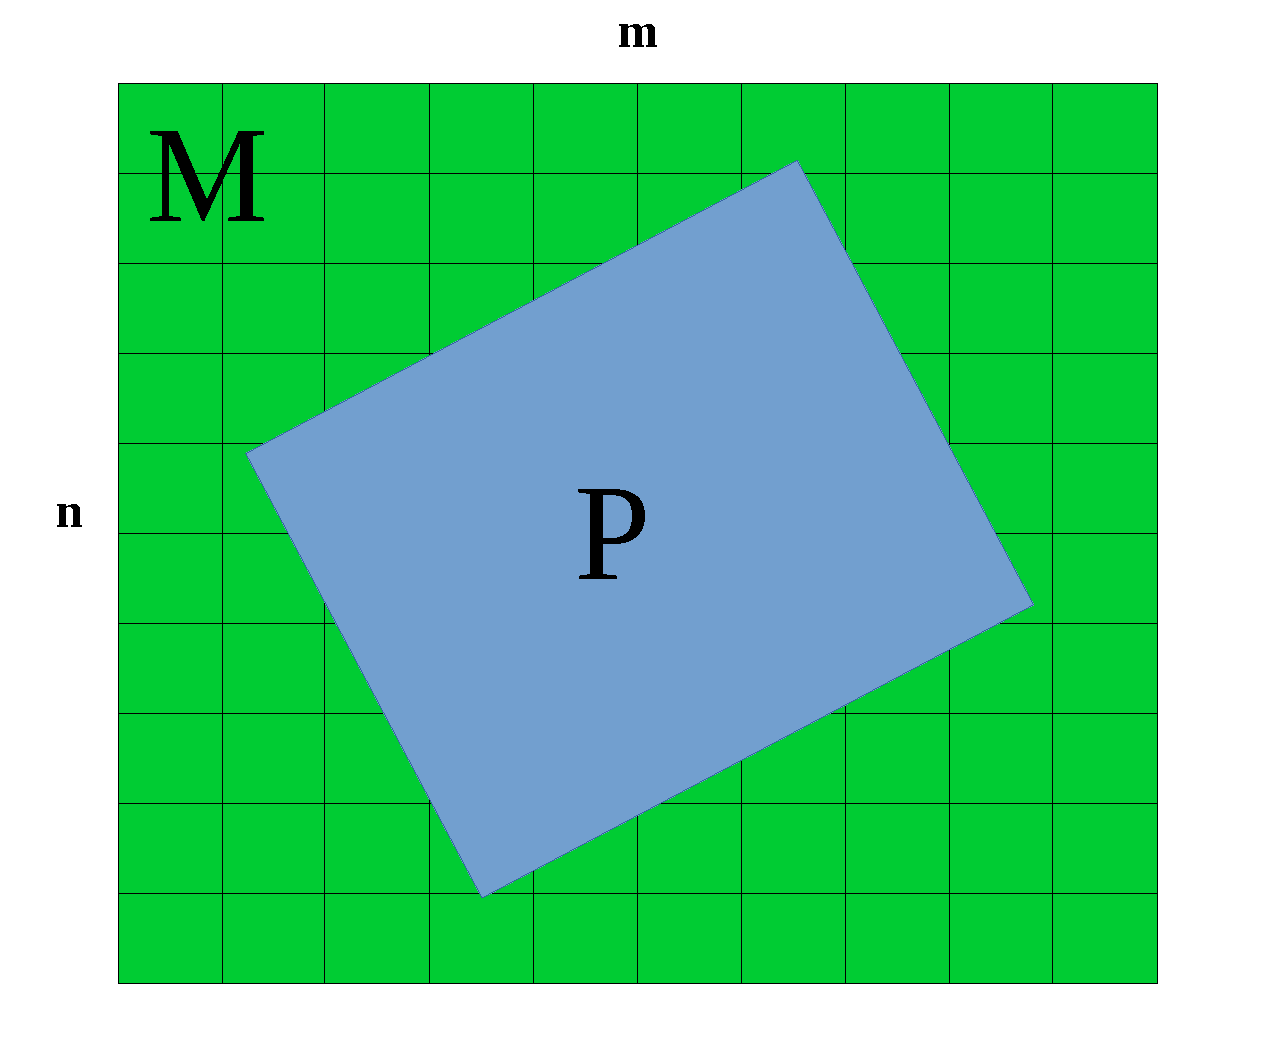
\includegraphics[ clip, scale=0.5]{mandf}}
	\centering
	\caption{blah}
	\label{fig:matrix_m}
\end{figure}
Załóżmy, że $p(x,y)$ jest funkcją mówiącą o tym czy punkt o współrzędnych $(x, y)$ znajduje się wewnątrz $P$. Jeśli $p = 0$ punkt należy do $P$, w przeciwnym wypadku $p=1$. Zraszacz jest definiowany jako okrąg reprezentowany przez promień $r_{i}$, współrzędne środka $(x_i, y_i)$ oraz konkretny model $t_{i}$. Środek każdego zraszacza musi zawierać się w $P$, czyli $p(x_{i}, y_{i}) = 0$.\\
Kwadrat o współrzędnych $(x,y)$ jest nawodniony jeśli znajduje się w zasięgu zraszacza. Jest to wyrażone następującą funkcją:
\begin{equation}
	is\_irr(x, y, s_{i}) = \begin{cases}
							1,& \text{jeśli } (x - x_{i})^{2} + (y - y_{i})^2 \leq r_{i}^{2}\\
							0,& w.p.p
						  \end{cases}
\end{equation}
, gdzie $x$ oraz $y$ oznaczają współrzędne środka kwadratu; $s_{i}$ jest konkretnym zraszaczem; $x_{i}, y_{i}$ oznaczają współrzędne zraszacza $s_{i}$; $r_{i}$ jest liczba wyrażającą zasięg zraszacza.\\\\
Załóżmy, że $S$ jest zbiorem wszystkich rozmieszczonych zraszaczy. Wtedy dany kwadrat jest nawodniony jeśli znajduje się w zasięgu przynajmniej jednego zraszacza ze zbioru $S$:
\begin{equation}
	irr(x, y, S) = \begin{cases}
				   	1,& \text{jeśli } \sum_{i=1}^{S} is\_irr(x,y,s_{i}) > 0 \\
				   	0,& w.p.p			   	
				   \end{cases}
\end{equation}
Generalnie poprzez stopień nawodnienia danego obszaru rozumie się różnicę pomiędzy liczbą wszystkich elementów macierzy $M$ należących do $P$, a liczbą nawodnionych elementów tej macierzy należących do $P$:
\begin{equation}\label{eq:simple_f1}
	F_{0}(S) = \sum_{m=1}^{M}\sum_{n=1}^{N} p(m,n) \cdot (1 - irr(m,n,S))
\end{equation}
Im wartość funkcji $F_{0}$ jest mniejsza tym mniej jest obszarów nienawodnionych, a więc rozwiązanie jest lepsze. $F_{0} = $ jest rozwiązaniem idealnym z perspektywy kryterium nawodnienia.\\\\
Jak zostało wspomniane w poprzednich rozdziałach zaimplementowane algorytmy oceniają stopień nawodnienia obszaru na dwa sposoby w zależności od tego czy wybrana jest opcja minimalizacji nawodnienia poza wskazanym obszarem. Jeśli minimalizacja jest wyłączona do obliczeń używana jest prosta funkcja opisana powyżej \eqref{eq:simple_f1}. Bardziej szczegółowe rozwinięcie funkcji przewiduje wprowadzenie kary za naruszenie ograniczeń:

\begin{equation}
\begin{split}
	F_{1}(S) = \sum_{m=1}^{M}\sum_{n=1}^{N} p(m,n) \cdot (1 - irr(m,n,S)) \\ + 
	\alpha \cdot \bigg{[}\dfrac{\sum_{m=1}^{M}\sum_{n=1}^{N} (1 - p(m,n)) \cdot irr(m,n,S) \cdot 100}{\sum_{m=1}^{M}\sum_{n=1}^{N} p(m,n)} \\ + \dfrac{\sum_{m=1}^{M}\sum_{n=1}^{N} p(m,n) \cdot ovrirr(m,n,S) \cdot 100}{\sum_{m=1}^{M}\sum_{n=1}^{N} p(m,n)}\bigg{]}
\end{split}
\end{equation}
, gdzie $\alpha$ jest zmienną określającą to czy na funkcję celu wpływa minimalizacja nawodnienia poza wskazanym obszarem. Zmienna $\alpha$ może przyjmować wartość 0 lub 1. Jeśli $\alpha=1$ minimalizacja jest brana pod uwagę; $ovrirr(m,n,S)$ jest funkcją mówiącą czy dany obszar został nadmiernie nawodniony \eqref{eq:is_overirrigated_func}.
\begin{equation}\label{eq:is_overirrigated_func}
	ovrirr(x,y,S) = \begin{cases}
				1,& \text{jeśli } \sum_{i=1}^{S} is\_irr(x,y,s_{i}) > 1 \\
				0,& w.p.p
			   \end{cases}
\end{equation}
\\Jak zostało wspomniane wcześniej, każdy rozmieszczony zraszacz charakteryzowany jest przez konkretny model. Załóżmy, że $C(t_{i})$ jest funkcją zwracającą cenę rynkową dla danego modelu $t_i$. Wtedy całkowity koszt konkretnego rozwiązania wynosi:
\begin{equation}
	F_{2}(S) = \sum_{i=1}^{S} C(t_{i})
\end{equation}\\
Podsumowując celem zadania jest rozwiązanie następującego problemu optymalizacyjnego:

\begin{equation}
	\begin{split}
		min \text{  } & 	F_{1}(S) = \sum_{m=1}^{M}\sum_{n=1}^{N} p(m,n) \cdot (1 - irr(m,n,S)) \\ +& 
		\alpha \cdot \bigg{[}\dfrac{\sum_{m=1}^{M}\sum_{n=1}^{N} (1 - p(m,n)) \cdot irr(m,n,S) \cdot 100}{\sum_{m=1}^{M}\sum_{n=1}^{N} p(m,n)} \\ +& \dfrac{\sum_{m=1}^{M}\sum_{n=1}^{N} p(m,n) \cdot ovrirr(m,n,S) \cdot 100}{\sum_{m=1}^{M}\sum_{n=1}^{N} p(m,n)}\bigg{]}\\\\
		min \text{  }&	F_{2}(S) = \sum_{i=1}^{S} C(t_{i})
	\end{split}
\end{equation}

\chapter{Optymalizacja}
Optymalizacja jest procesem polegającym na wyznaczeniu najlepszego rozwiązania lub rozwiązań z punktu widzenia danego kryterium lub kryteriów. Procesy takie w w obecnym świecie obecne są wszędzie. Zaczynając od mechaniki, poprzez ekonomie, finanse, elektrykę po geofizykę czy modelowanie molekularne. Przykładem może być konieczność minimalizacji kosztów produkcji w fabryce, maksymalizacja prawdopodobieństwa zysku z przeprowadzanych transakcji czy chociażby znalezienie najbardziej odpowiadającego danej osobie modelu samochodu.

W kolejnych podrozdziałach dokładnie opisane zostaną zagadanie powiązane kolejno z optymalizacją jednokryterialną oraz wielokryterialną.
\section{Optymalizacja jednokryterialna}
Optymalizacja jednokryterialna, jak wskazuje nazwa, odnosi się do problemów opisywanych za pomocą jednej funkcji celu. Przykładem może być tutaj problem spotykający ludzi wybierających się na wakacje, a więc poszukiwanie najlepszego hotelu w danym mieście. Załóżmy, że jedynym kryterium branym pod uwagę w trakcie szukania takiego hotel jest cena ze spęrdzoną noc. Przykładem będzie tutaj sytuacja przestawiona na rysuku \eqref{fig:opt_ex}. Jak łatwo zauważyć najtańszy jest hotel $A$. Można więc powiedzieć, że hotel $A$ jest rozwiązaniem przedstawionego problemu optymalizacyjnego. Patrząc na to z drugiej strony, możemy stwierdzić, że cena hotelu nie ma dla nas żadnego znaczenia, a zależy nam jedynie na tym aby ten znajdował się jak najbliżej morza. Przy takiej zmianie kryterium, zmienia się również rozwiązanie problemu. Najlepszy staje się hotel $E$, ponieważ to właśnie on znajduje się najbliższej morza.

Z matematycznego punktu widzenia rozwiązanie jednokryterialnego problemu optymalizacyjnego sprowadza się do znalezienia ekstremum  funkcji opisującej wybrane kryterium oceny.
\begin{figure}[!htb]
	\makebox[\textwidth]{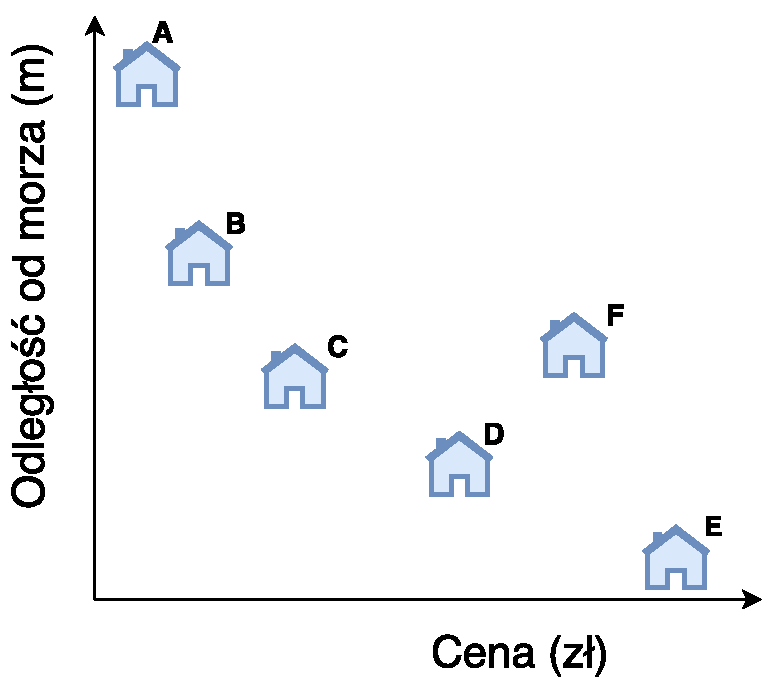
\includegraphics[ clip, scale=0.6]{opt_ex}}
	\centering
	\caption{Powiązanie pomiędzy ceną hotelu, a dystansem od morza}
	\label{fig:opt_ex}
\end{figure}
\section{Optymalizacja wielokryterialna}
Jeśli problem optymalizacyjny zawiera w sobie kilka funkcji celu, proces znajdowania optymalnego rozwiązania bądź rozwiązań nazywa się optymalizacją wielokryterialną. Zdecydowana większość realnych problemów jest właśnie przykładem wymagającym wykorzystania optymalizacji wielokryterialnej. W takich przypadkach nie można skupiać się jedynie na jednym kryterium, ponieważ pozostałe są równie ważne. Przykładem może być tutaj problem wyboru hotelu na wakacje, opisany w poprzednim podrozdziale. 

Załóżmy, że tym razem oba kryteria przedstawione na rysunku \eqref{fig:opt_ex} są dla nas tak samo ważne. Gdyby było inaczej i wszyscy kierowali by się jedynie ceną hotelu, wszyscy chcieliby mieszkać w hotelu $A$. Oczywiście w realnym świecie taka sytuacja nigdy nie będzie miała miejsca, ponieważ w większości przypadków proces decyzyjny nie jest taki prosty.

Jak możemy zauważyć do wyboru mamy 6 różnych hoteli. Każdy z nich charakteryzuje się ceną za jedną noc oraz odległością od morza wyrażoną w metrach. Do porównania wybierzmy dwa hotele: $D$ oraz $F$. Jak widać hotel $D$ jest zarówno tańszy jak i znajduje się bliżej morza w porównaniu do hotelu $F$. W tym przypadku decyzja o wyborze jest oczywista i jest nią hotel $D$. Sytuacja wygląda inaczej, gdy porównamy hotel $D$ z hotelem $C$. Hotel $D$ znajduję się bliżej plaży, natomiast jest również droższy od $C$. Które rozwiązanie w tej sytuacji będzie lepsze? To już zależy wyłącznie od preferencji konkretnej osoby. Nie da się bowiem stwierdzić, które z wybranych rozwiązań jest lepsze patrząc z perspektywy obu kryteriów. Z tego powodu problemy, w których występuje kilka kryteriów negatywnie na siebie wpływających, charakteryzują się posiadaniem wielu rozwiązań optymalnych.

\subsubsection{Dominacja}
Jednym z głównych pojęć, na których opiera się optymalizacja wielokryterialna jest pojęcie dominacji. Jednym z celów rozwiązywania problemów wielokryterialnych jest znalezienie rozwiązań niezdominowanych, co dokładniej wyjaśnione zostanie później. Koncept dominacji polega na porównywaniu ze sobą znalezionych rozwiązań przez pryzmat wszystkich określonych kryteriów oceny. Załóżmy, że $M$ określa liczbę kryteriów. Wtedy można powiedzieć, że rozwiązanie $A$ dominuje rozwiązanie $B$ jeśli:\\

\begin{enumerate}
	\item Dla każdego kryterium $m \in M$ rozwiązanie $A$ nie jest gorsze od $B$.
	\item Przynajmniej dla jednego kryterium $m \in M$ rozwiązanie $A$ jest lepsze od $B$.\\
\end{enumerate}

Korzystając z przykładu opisanego wcześniej przykładu hoteli, możemy zauważyć, że rozwiązanie $F$ jest zdominowane przez rozwiązanie $D$. Jest tak dlatego, że rozwiązanie $D$ jest pod względem każdego kryterium lepsze od rozwiązania $F$, a więc spełnione są wymienione powyżej warunki. Nie można tego samego powiedzieć, gdy do porównania użyjemy hotelu $A$ oraz $B$. Rozwiązanie $A$ nie spełnia pierwszego warunku - hotel jest położony dalej od morza.

\subsubsection{Optimum Pareto}
Rozwiązanie jest rozwiązaniem optymalnym w sensie Pareto, jeśli nie da się poprawić danego rozwiązania pod względem jednego kryterium, nie pogarszając jednocześnie oceny rozwiązania, patrząc z perspektywy pozostałych kryteriów. Spójrzmy na hotel $C$ z wykorzystywanego wcześniej przykładu oraz załóżmy, że jest to rozwiązanie optymalne w sensie Pareto. W takiej sytuacji nie da obniżyć się ceny za pobyt w hotelu bez zmiany jego lokalizacji, oddalającej go od plaży. Sytuacja wygląda identycznie w drugą stronę. Nie da się zmienić położenia hotelu na bliższe morzu, bez zwiększenia ceny za noc. Optimum Pareto jest więc kompromisem pomiędzy pomiędzy uwzględnianymi kryteriami.

Grupa rozwiązań optymalnych w sensie Pareto tworzy tzw. front lub zbiór Pareto. Rozwiązanie optymalne w sensie Pareto jest jednocześnie rozwiązaniem niezdominowanym, tak więc front Pareto jest również zbiorem rozwiązań niezdominowanych. Przykład takiego frontu, w postaci niebieskiej linii, został przestawiony na rysunku \eqref{fig:pareto_ex}. Rozwiązania (1-4) leżące na froncie są rozwiązaniami optymalnymi w sensie Pareto, które dominują pozostałe rozwiązania znajdujące się na rysunku.
\begin{figure}[!htb]
	\makebox[\textwidth]{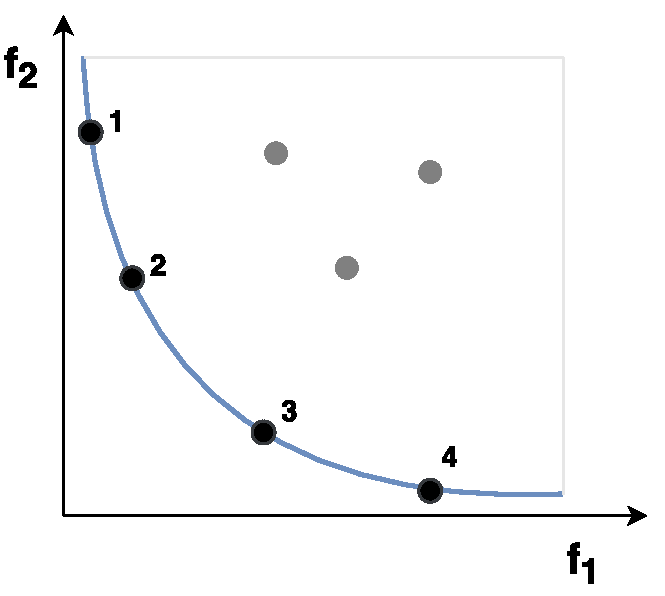
\includegraphics[ clip, scale=0.5]{pareto_ex}}
	\centering
	\caption{Front Pareto}
	\label{fig:pareto_ex}
\end{figure}

Przedstawiona powyżej definicja frontu Pareto może zostać wykorzystana w dwóch kontekstach: lokalnym oraz globalnym. Front Pareto w sensie globalnym jest zbiorem rozwiązań niezdominowanych w kontekście całej przestrzeni możliwych rozwiązań. Lokalny front Pareto natomiast, jest grupą rozwiązań niezdominowanych ale tylko w określonym zakresie przestrzeni. Biorąc to pod uwagę dowolną grupę rozwiązań można podzielić na $n$ frontów, gdzie $n$ jest liczbą frontów potrzebnych do objęcia wszystkich rozwiązań z grupy. Zostało to zobrazowane na rysunku \eqref{fig:fronts_ex}. Liczby znajdujące się przy frontach oznaczają ich miejsce w hierarchii. Najlepszy front oznaczony jest liczbą 1, kolejny liczbą 2 itd.. Warto tutaj zauważyć, że rozwiązania znajdujące się na drugim froncie nie są niezdominowane w sensie globalnym (dominują je rozwiązania z frontu pierwszego). Są natomiast optymalne w sensie lokalnym, czyli po ograniczeniu przestrzeni rozwiązań do tych nieznajdujących się na pierwszym froncie.
\begin{figure}[!htb]
	\makebox[\textwidth]{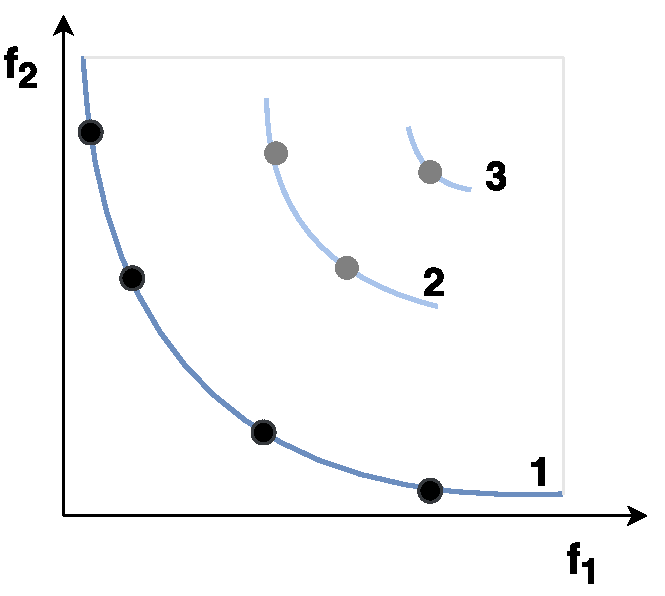
\includegraphics[ clip, scale=0.6]{fronts_ex}}
	\centering
	\caption{Lokalne fronty Pareto}
	\label{fig:fronts_ex}
\end{figure}
\subsubsection{Sortowanie rozwiązań niezdominowanych}
Proces podziału dostępnych rozwiązań na fronty nazywa się sortowaniem rozwiązań niezdominowanych. Jest to ważne zagadnienie, ponieważ często wykorzystywane jest w metodach optymalizacji wielokryterialnej.

\chapter{Algorytmy genetyczne}
Problem optymalizacyjny opisany na wstępie pracy został rozwiązany przy użyciu algorytmów genetycznych. Są to algorytmy, których działanie oparte jest na tych samych zasadach na których odbywa się proces ewolucji zachodzący w naturze. W tym rozdziale przedstawiony zostanie opis ogólny algorytmu genetycznego, jego powiązanie z procesami zachodzącymi w przyrodzie, schemat działania oraz dokładny opis wykorzystywanych operatorów: krzyżowania, selekcji oraz mutacji. Następnie przedstawiony zostanie koncept wielokryterialnych algorytmów genetycznych oraz opisane zostaną dwa algorytmy wykorzystane do rozwiązania przedstawionego wcześniej problemu: NSGA-II oraz SPEA. Kolejny podrozdział będzie skupiał się na procesie strojenia algorytmów. Następnie opisana zostanie konkretna implementacja zastosowana w celu rozwiązania problemu nawodnienia.
\section{Opis ogólny}
Algorytmy genetyczne są procedurami wykorzystywanymi do rozwiązywania problemów optymalizacyjnych, opartymi o genetykę oraz selekcję naturalną. Cały proces działania takiego algorytmu można porównywać do procesu ewolucji występującego w przyrodzie. Obserwując taki proces można zauważyć, że najlepiej przystosowane osobniki mają największe szanse na reprodukcję, a więc przekazanie swojego DNA kolejnym pokoleniom. Dzieje się tak dlatego, że z punktu widzenia biologii najlepiej przystosowane osobniki to te najbardziej atrakcyjne dla potencjalnych partnerów oraz w przypadku zwierząt stadnych, te dominujące całą resztę, a więc mające pierwszeństwo jeśli chodzi o wybór partnerów, reprodukcję czy chociażby pożywianie się. Generalizując natura dąży do tego, aby do puli z której utworzone ma zostać kolejne pokolenie danej populacji trafiały jak najlepsze geny. Gdyby działo się inaczej żaden gatunek nie przetrwałby więcej niż kilkudziesięciu pokoleń.\\
Jak zostało wspomniane największe szanse na potomstwo mają osobniki najlepsze patrząc z perspektywy szansy na przetrwanie. Potomstwo par takich osobników powstaje na skutek procesu nazywanego krzyżowaniem. Krzyżowanie polega na łączeniu genów jednego osobnika z drugim, tworząc w ten sposób potomka, charakteryzującego się cechami zarówno pierwszego jak i drugiego rodzica. Oczywiście im lepiej rodzice danego osobnika byli przystosowani, tym większa szansa, że również i on będzie stał wysoko w hierarchii.\\
Kolejnym istotnym elementem w procesie ewolucji jest mutacja. Mutacja jest losowym procesem polegającym na zmianie fragmentu kodu DNA. Poprzez taką zmianę osobnik staje się jeszcze lepiej lub gorzej przystosowany. W pierwszym przypadku jego szanse na reprodukcję wzrastają, więc jest większe prawdopodobieństwo, że zmiana wprowadzona przez mutację zostanie przekazana dalej. W drugim przypadku linia osobników ze zmienionym DNA prawdopodobnie wygaśnie zdecydowanie szybciej niż w przypadku pierwszym.

Podsumowując, proces ewolucji złożony jest z trzech elementów: selekcji, krzyżowania oraz mutacji. Na tych samych operacjach opiera się działanie algorytmu genetycznego. W kontekście algorytmu są one nazywane operatorami genetycznymi. Na rysunku \eqref{fig:ga_sequence} przedstawiony został ogólny schemat działania takiego algorytmu.
\begin{figure}[!htb]
	\makebox[\textwidth]{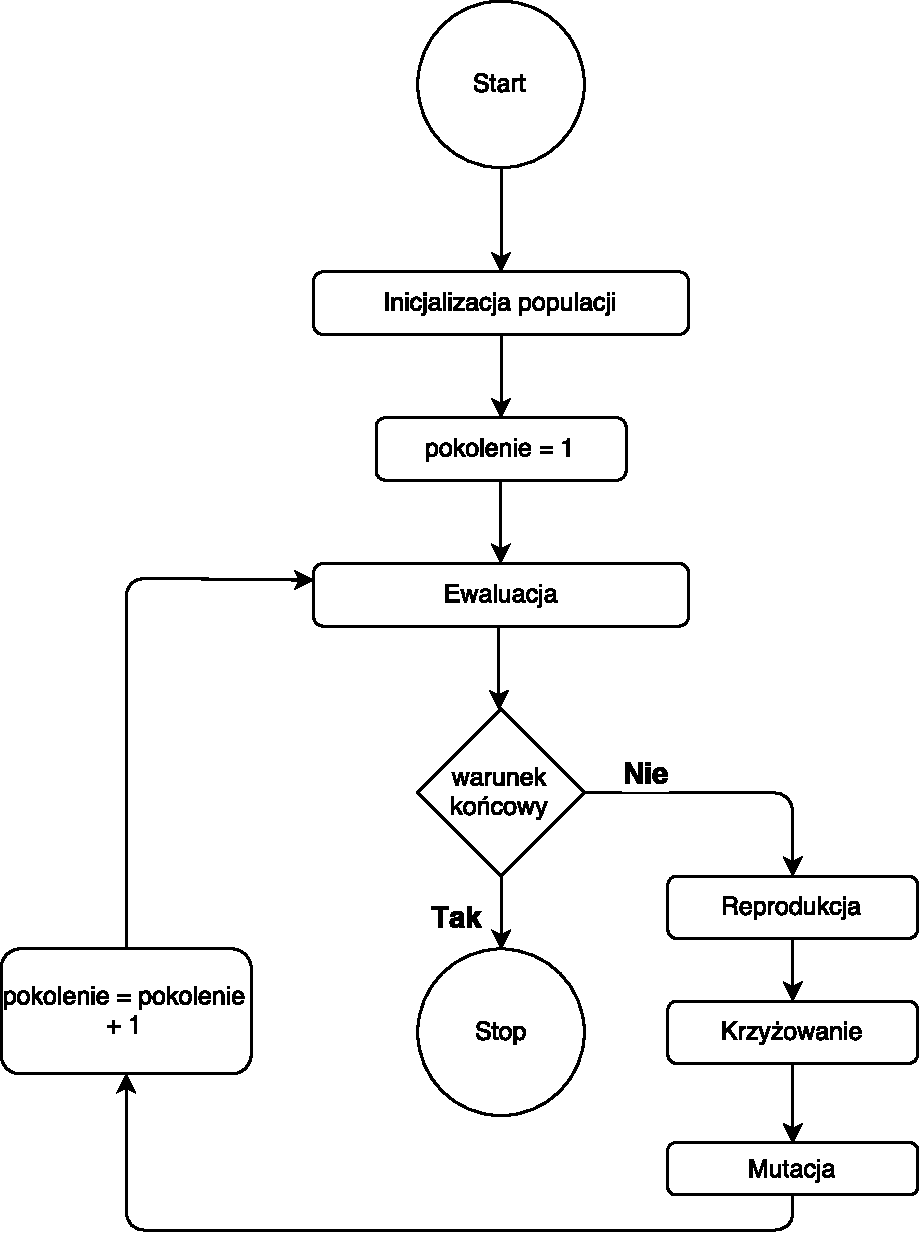
\includegraphics[ clip, scale=0.5]{ga_sequence}}
	\centering
	\caption{Schemat działania algorytmu genetycznego}
	\label{fig:ga_sequence}
\end{figure}

Punktem startowym jest utworzenie losowej populacji osobników. Następnie każdy osobnik jest oceniany przez pryzmat ustalonego kryterium. Na podstawie oceny przeprowadzany jest proces selekcji, czyli wyboru najlepszych osobników, które wykorzystane zostaną do reprodukcji. Podczas procesu reprodukcji generowane są nowe osobniki tworzące kolejne pokolenie. Każdy nowy osobnik jest wynikiem krzyżowania, czyli łączenia chromosomu dwóch rodziców w jeden. Chromosom z punktu widzenia biologii jest formą organizacji materiału genetycznego. Z punktu widzenia algorytmu będzie to zestaw parametrów charakteryzujących danego osobnika, który zostanie opisany później. Następnie chromosomy nowych osobników mogą ulec mutacji, czyli losowej zmianie pojedynczych genów. Gdy zostanie utworzona odpowiednia liczba nowych osobników, czyli powstanie nowe pokolenie, cały proces zaczyna się od początku, dopóki nie osiągnięte zostanie zdefiniowane kryterium końcowe.\\\\
W powyższym opisie pojawiło się kilka pojęć wartych wyjaśnienia.
\subsubsection{Populacja}
Populacja jest grupą o ustalonym rozmiarze. Elementami grupy są pojedyncze osobniki. Jedną z przewag algorytmów genetycznych nad tradycyjnymi technikami optymalizacyjnymi jest właśnie operowanie nie na jednym konkretnym rozwiązaniu, lecz na całej grupie. Duża różnorodność osobników w połączeniu z odpowiednim użyciem operatorów genetycznych pozwala uniknąć problemu utknięcia na optimum lokalnym.
\subsubsection{Chromosom}
Chromosom, jak zostało już wspomniane, jest sposobem reprezentacji właściwości cechujących danego osobnika. Chromosom można zdefiniować na dwa sposoby: za pomocą ciągu binarnego lub wartości rzeczywistych. Ciąg binarny jest ciągiem wartości $0$ lub $1$ ułożonych w taki sposób aby odpowiednio zakodować przekazywaną informację. W ramach przykładu załóżmy, że mamy dany cylinder o średnicy $d = 10 cm$ oraz wysokości $h = 14 cm$. Rysunek \eqref{fig:cylinder} pokazuje przykładowy sposób reprezentacji takiego cylindra w formie ciągu binarnego. 
\begin{figure}[!htb]
	\makebox[\textwidth]{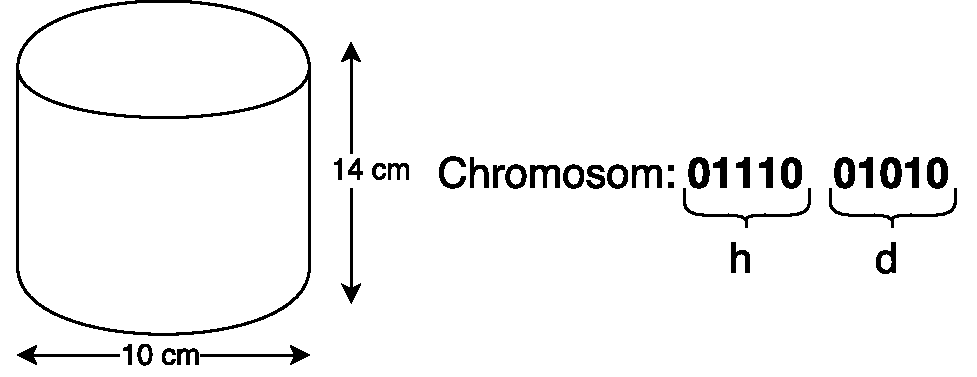
\includegraphics[ clip, scale=0.5]{cylinder}}
	\centering
	\caption{Przykład ciągu binarnego}
	\label{fig:cylinder}
\end{figure}
\\Chromosom reprezentujący cylinder złożony jest z 10 bitów. Na pierwszych pięciu z nich zakodowana jest informacja o wysokości, a na kolejnych informacja o średnicy. Wartości przedstawione przez poszczególne części ciągu należy traktować jak liczby binarne i w ten sam sposób je interpretować.

W większości przypadków preferowane jest używanie ciągu binarnego jako sposobu reprezentacji osobników. Jednym z powodów jest łatwość przeprowadzania operacji krzyżowania oraz mutacji, o których mowa będzie później. Używając reprezentacji binarnej można w prosty sposób zmienić sposób kodowania osobników bez konieczności ingerowania w operatory genetyczne - operatory krzyżowania oraz mutacji nie biorą pod uwagę sposobu w jaki informacja została zapisana w chromosomie. Kolejne argumenty przemawiające za użyciem takiej reprezentacji przedstawione zostały w pracach Hollanda (1991)REF oraz Goldberga (1993)REF. Kolejne etapy działania algorytmów genetycznych wyjaśnione zostaną przy założeniu, że osobniki przedstawione są za pomocą ciągów binarnych.
\subsubsection{Ewaluacja}
Po ustaleniu sposobu reprezentacji osobników należy wygenerować losową populację oraz poddać ją ocenie, czyli ewaluacji. Proces ewaluacji polega na przypisaniu każdemu osobnikowi odpowiedniej wartości pozwalającej ocenić go na tle reszty populacji. Jest to wartość dopasowania osobnika. Korzystając z wcześniejszego przykładu załóżmy, że podczas procesu ewaluacji zdefiniowanemu wcześniej cylindrowi przypisywany jest koszt wyprodukowania, wyrażony następującym wzorem:
\begin{equation}
f(d,h) = c\big{(}\dfrac{\pi d^{2}}{2} + \pi dh\big{)}
\end{equation}
, gdzie $c$ oznacza koszt materiału na $cm^{2}$.\\
Zgodnie z podanymi wcześniej danymi oraz przy założeniu, ze $c = 0.01$ koszt wyprodukowania danego cylindra wynosi:
\[f(10, 14) = 6\]
Zakładając, że celem procesu optymalizacji jest minimalizacja kosztu wyprodukowania cylindra, należy zauważyć, że osobnik z przypisaną mniejszą wartością jest lepszy w kontekście wybranego kryterium.
\subsubsection{Reprodukcja}
Kolejnym etapem działania algorytmu genetycznego jest reprodukcja inaczej zwana też selekcją. Jest to proces mający na celu zwiększenie liczby dobrych osobników w populacji oraz redukcję liczby tych gorszych, jednocześnie utrzymując niezmieniony rozmiar całej populacji. Jest to osiągane poprzez realizację następujących zadań:\\
\begin{enumerate}
	\item Zidentyfikowanie dobrych (ocenionych powyżej średniej) osobników.
	\item Utworzenie kopii dobrych osobników.
	\item Eliminacja osobników gorszych, tak aby kopie dobrych mogły zostać dodane do populacji.\\
\end{enumerate}
Powyższe zadania mogą zostać osiągnięte przy użyciu kilku metod. Najpopularniejszymi z nich są: metoda turniejowa, metoda ruletki oraz metoda rankingu.
Metoda turniejowa polega na rozgrywaniu turniejów pomiędzy kilkoma osobnikami wybranymi losowo z populacji. Zwycięzca każdego turnieju, jako rodzic, przechodzi do etapu krzyżowania, który zostanie opisany później\eqref{fig:tournament}. Rozmiar pojedynczego turnieju znacząco wpływa na przebieg procesu selekcji. Im jest większy, tym mniejsza szansa, że słabsze osobniki przejdą do kolejnego etapu. Wbrew pozorom takie zachowanie nie jest pożądane ze względu na potrzebę zachowania różnorodności populacji. Im rozmiar jest większy tym większa szansa, że do kolejnego etapu dostanie się zbyt dużo słabszych osobników, co również nie jest dobrym rozwiązaniem. Jeśli rozmiar turnieju $S = 1$ selekcja staje się równoważna losowemu wyborowi osobnika. Najczęściej stosuje się turnieje o rozmiarze 2. Metoda turniejowa jest jedną z najczęściej wybieranych metod selekcji. Jest prosta w implementacji oraz pozwala na łatwe manipulowanie rozmiarem turnieju, co z kolei wpływa na szybkość zbliżania się znalezionych rozwiązań do rozwiązania optymalnego. Ponadto jak zostało udowodnione selekcja turniejowa zawsze zapewnia lepszą lub taką samą szybkość zbliżania się do rozwiązań optymalnych jak inne metody selekcji oraz mniejszą lub taką samą złożoność obliczeniową. Z wymienionych powyżej powodów to właśnie metoda turniejowa została zaimplementowana w wybranych przez autora algorytmach.
\begin{figure}[!htb]
	\makebox[\textwidth]{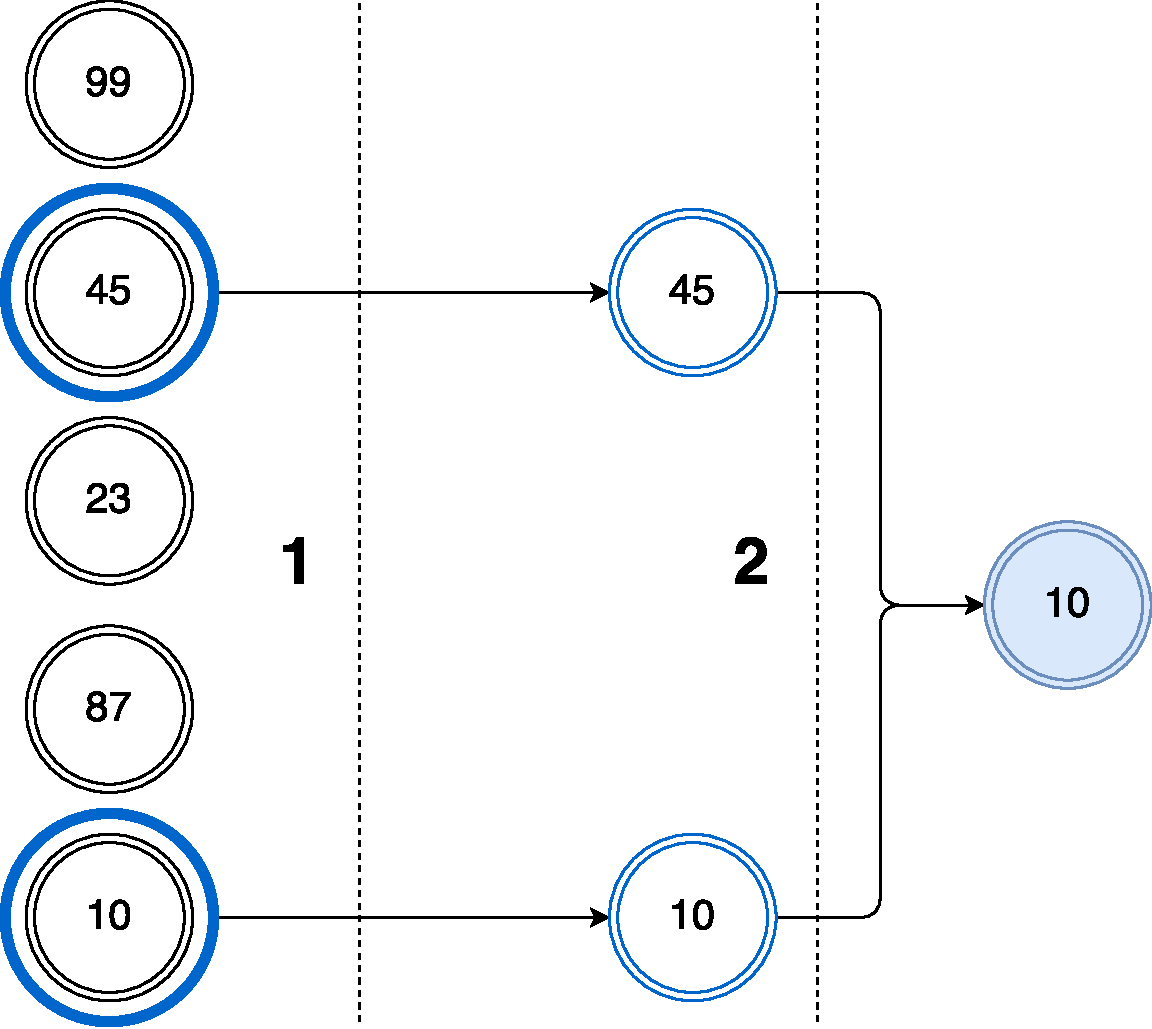
\includegraphics[ clip, scale=0.5]{tournament}}
	\centering
	\caption{Przykład rozegranego turnieju o rozmiarze 2.\\1.Wybór losowych osobników; 2.Turniej pomiędzy wybranymi osobnikami.}
	\label{fig:tournament}
\end{figure}

Kolejną popularną metody selekcji jest metoda proporcjonalna. W metodzie tej wprowadzone zostaje pojęcie puli rozrodczej. Jest to pula spośród której wybierane są osobniki wykorzystywane później do krzyżowania. Wypełnienie puli rozrodczej kopiami osobników wykonywane jest procesie selekcji. Liczba kopii danego osobnika w puli jest proporcjonalna do jego wartości dopasowania. Jeśli średnia wartość dopasowania dla całej populacji wynosi $f_{avg}$, dany osobnik $s_{i}$ będzie posiadał $f_{i}/f_{avg}$ kopii w puli rozrodczej. Metoda proporcjonalna często nazywana jest również metodą ruletki, ponieważ właśnie za pomocą koła ruletki można zobrazować sobie jej działanie. Wspomniane koło jest podzielone na $N$ części, gdzie $N$ jest wielkością populacji. Każdy wycinek koła odpowiada jednemu osobnikowi z populacji. Wielkość danego wycinka jest proporcjonalna do wartości dopasowania osobnika. Wynika z tego, że wycinki powiązane z lepszymi osobnikami będą zajmować większą część koła. Jak można zauważyć na rysunku \eqref{fig:roulette} osobnik o numerze 6 jest najlepszy na tle całej populacji, natomiast osobnik o numerze 2 jest osobnikiem najgorszym. Wybór osobników do puli rozrodczej odbywa się poprzez kręcenie kołem. Czynność ta powtarzana jest $N$ razy. Po zatrzymaniu wybierany jest osobnik na którego wycinku zatrzymał się wskaźnik. Osobniki z najlepszą wartością dopasowania mają największe szanse na trafienie do puli rozrodczej.

Wadami metody proporcjonalnej jest duża złożoność obliczeniowa oraz problemy ze skalowaniem. Załóżmy, że jeden osobnik jest znacząco lepszy od reszty. Wtedy powiązany z nim wycinek będzie zajmował niemal całe koło, a co za tym idzie prawdopodobieństwo wyboru takiego osobnika będzie zbliżone do 1. W konsekwencji pula rozrodcza będzie w większości zapełniona kopiami jednego osobnika, co prowadzi do braku zróżnicowania. Z drugiej strony jeśli wszystkie osobniki mają bardzo zbliżone wartości dopasowania, każdy z nich ma również podobne prawdopodobieństwo wyboru do puli. Prowadzi to do sytuacji, kiedy każdy osobnik ma dokładnie jedną kopię w puli rozrodczej. Taki proces selekcji nie wnosi żadnej wartości i równie dobrze mógłby zostać pominięty. 
\begin{figure}[!htb]
	\makebox[\textwidth]{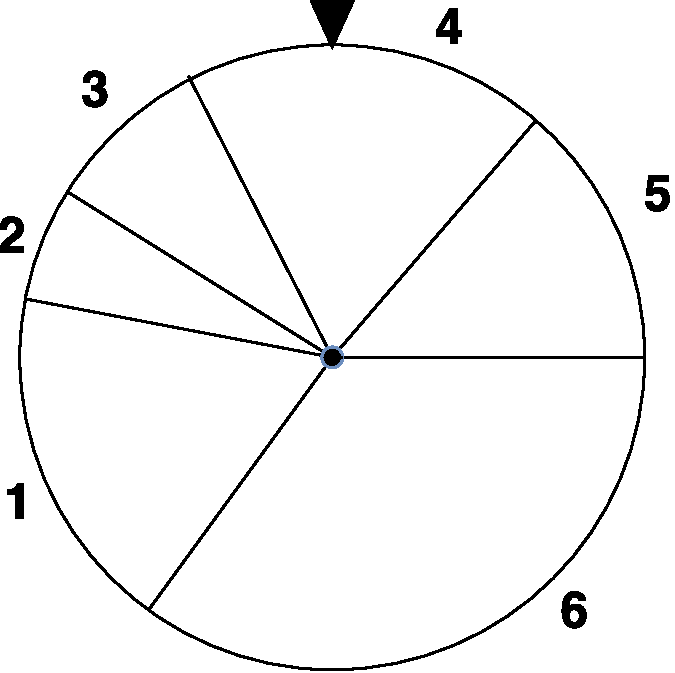
\includegraphics[ clip, scale=0.5]{roulette}}
	\centering
	\caption{Przykładowa wizualizacja selekcji proporcjonalnej}
	\label{fig:roulette}
\end{figure}

Opisanych powyżej problemów ze skalowaniem można uniknąć korzystając z metody rankingowej. Polega ona na posortowaniu osobników z populacji ze względu na ich wartość dopasowania. W ten sposób najgorszemu osobnikowi zostaje przypisane pierwsze miejsce w tworzonym rankingu. Osobnik najlepszy znajdzie się wtedy na $N$-tym miejscu. Po takim przygotowaniu na posortowanej populacji zostaje użyty operator selekcji proporcjonalnej. Na tym etapie przygotowanie koła ruletki nie opiera się już na wartości dopasowania poszczególnych osobników, lecz na ich pozycji w rankingu. Pozwala to na pozbycie się opisanych wcześniej problemów.

\subsubsection{Krzyżowanie}
Po wyborze osobników mających zostać rodzicami następuje czas na skorzystanie z operatora krzyżowania. Tutaj należy zwrócić uwagę na to, że opisany wcześniej proces reprodukcji nie tworzy żadnych nowych osobników. Dzieje się to dopiero w trakcie procesu krzyżowania. Jak wskazuje nazwa, krzyżowanie polega na łączeniu dwóch osobników w celu utworzenia ich potomstwa. Dzieje się to na poziomie zdefiniowanych wcześniej chromosomów. Najprostszą i najlepiej ilustrującą ideę krzyżowania metodą jest metoda jednopunktowa. Polega ona na losowym wybraniu punktu względem którego nastąpi podział chromosomu na dwie części. Potomstwo powstaje na skutek wymiany pomiędzy rodzicami części chromosomu znajdującej się po prawej stronie od wybranego punktu podziału. Proces ten został przedstawiony na rysunku \eqref{fig:one_point_cross}. Po lewej stronie znajdują się chromosomy pary rodziców. Punkt podziału został losowo ustalony na $d=4$, co symbolizuje pionowa przerywana linia. Po prawie stronie znajduje się potomstwo - wynik zastosowania operatora krzyżowania. Jak widać chromosom każdego nowego osobnika powstał na skutek złożenia chromosomów rodziców.
\begin{figure}[!htb]
	\makebox[\textwidth]{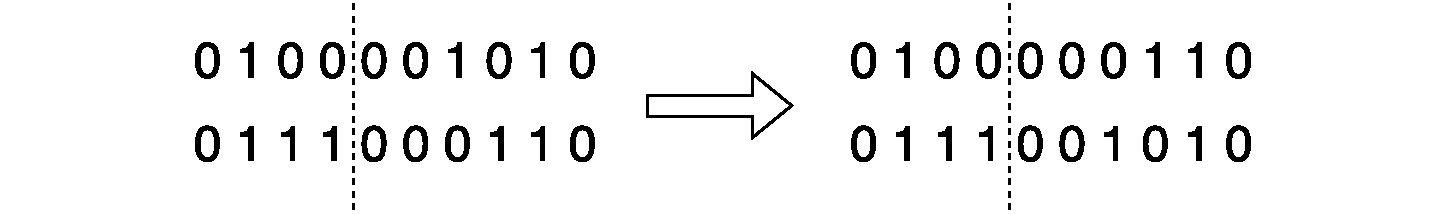
\includegraphics[ clip, scale=0.34]{one_point_cross}}
	\centering
	\caption{Przykład krzyżowania jednopunktowego}
	\label{fig:one_point_cross}
\end{figure}

W tym miejscu należy zauważyć, że nowe osobniki utworzone w procesie krzyżowania niekoniecznie muszą być lepsze od swoich rodziców. Może zdarzyć się tak, że potomstwo będzie gorzej przystosowane. Nie należy się tym jednak martwić, ponieważ jak zostało wyjaśnione wcześniej osobniki o mniejszej wartości przystosowania mają mniejsze szanse na przetrwanie selekcji, a co za tym idzie ich geny nie zostaną przekazane kolejnym pokoleniom. Ponadto jest znacznie bardziej prawdopodobne, że operatory krzyżowania wygenerują rozwiązania lepsze niż generowanie losowe. Dzieje się tak dlatego, że chromosomy wybrane do procesu nie są przypadkowe. Przeszły one selekcje co wskazuje na to, że zawierają w sobie wartościowe kombinacje bitów. Operator krzyżowania użyty na parze rodziców, może wygenerować jedynie $l$ par potomków, gdzie $l$ jest długością chromosomu. Biorąc pod uwagę fakt, że potomstwo jest generowane przy użyciu chromosomów dobrych osobników, istnieje duże prawdopodobieństwo, że utworzone rozwiązania również będą dobre.

Opisany powyżej proces krzyżowania może zostać przeprowadzony również przy użyciu kilku punktów podziału. Na rysunku \eqref{fig:two_point_cross} przedstawiona jest selekcja dwupunktowa. Chromosom dzielony jest na trzy części. Potomstwo powstaje na skutek wymiany części środkowej.
\begin{figure}[!htb]
	\makebox[\textwidth]{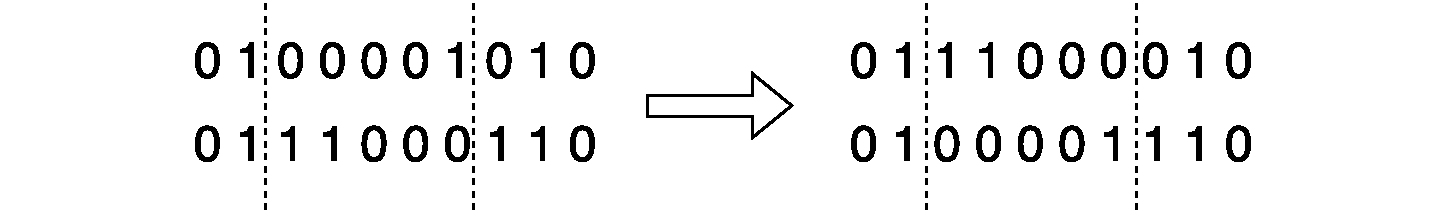
\includegraphics[ clip, scale=0.5]{two_point_cross}}
	\centering
	\caption{Przykład krzyżowania dwupunktowego}
	\label{fig:two_point_cross}
\end{figure}

Przedstawioną ideę podziału chromosomu można dowolnie rozszerzać. Ekstremum jest tzw. podział jednolity. W takim przypadku potomstwo powstaje poprzez wymianę pojedynczych bitów z określonym prawdopodobieństwem $p$. Najczęściej przyjmuje się, że $p = 0.5$, czyli istnieję 50\% szansy, że dany bit zostanie wymieniony na ten pochodzący z drugiego rodzica.

W wybranych algorytmach autor stosuje metodę krzyżowania dwupunktowego, która jest typowym wyborem przy chromosomach reprezentowanych za pomocą ciągów binarnych.

W celu zachowania części dobrych osobników z populacji, do procesu krzyżowania dodaje się dodatkową zmienną $p_{c}$, oznaczająca prawdopodobieństwo krzyżowania. Oznacza ona jaka część obecnej populacji zostanie użyta do procesu krzyżowania. Gdy $p_{c} = 1$ nowa populacja w całości zostanie zapełniona potomkami osobników ze starej populacji. W innym przypadku $100(1 - p_{c})\%$ osobników ze starej populacji zostanie skopiowanych do nowej. Najczęściej prawdopodobieństwo krzyżowania ustawia się na poziomie 80-90\%.
\subsubsection{Mutacja}
Nowe osobniki powstałe na skutek krzyżowania mogą ulec mutacji. Mutacja jest odpowiedzialna za losową modyfikację chromosomu danego osobnika. Operator mutacji zapewnia utrzymanie różnorodności populacji na odpowiednim poziomie. Działanie tego operatora opiera się na zmiennej wyrażającej prawdopodobieństwo mutacji: $p_{m}$. Operator nie działa na poziomie całego chromosomu, lecz pojedynczych bitów, a jego zastosowanie jest równoznaczne ze zmianą wartości danego bitu. Zostało to zilustrowane na rysunku \eqref{fig:mutation}.
\begin{figure}[!htb]
	\makebox[\textwidth]{
\includegraphics[ clip, scale=0.5]{mutation}}
	\centering
	\caption{Przykład mutacji}
	\label{fig:mutation}
\end{figure}

Podobnie jak w przypadku zastosowania operatora krzyżowania tak i w przypadku mutacji, osobnik będący rezultatem może okazać się gorszy od oryginału. Mimo to, warto zauważyć, że używanie operatora mutacji przy użyciu niskiego prawdopodobieństwa $p_{m}$ nie jest operacją losową. Powodem jest to, że rozwiązanie generowane jest na podstawie już istniejącego osobnika oraz cały proces może utworzyć jedynie kilka nowych rozwiązań, z dużym prawdopodobieństwem, również dobrych.\\

Podsumowując, algorytmy genetyczne używają trzech operatorów: selekcji, krzyżowania oraz mutacji. Operator selekcji odpowiedzialny jest za wybór najlepiej przystosowanych osobników. Operator krzyżowania służy do łączenia wybranych wcześniej osobników w celu utworzenia potomstwa. Operator mutacji losowo zmienia część chromosomu danego osobnika w nadziei na znalezienie jeszcze lepszego rozwiązania. Należy tutaj zwrócić uwagę, że żaden z opisanych operatorów nie jest deterministyczny. Każdy z nich oparty jest w znacznym stopniu o losowość, co powoduje, że nie zawsze będą one osiągać zamierzone rezultaty. Nie mniej jednak w kontekście działania algorytmu wymagane jest, aby gorsze osobniki były eliminowane w procesie reprodukcji, na rzecz osobników lepszych, których geny powinny być przekazywane do kolejnych pokoleń.
\section{Algorytmy wielokryterialne}
Główną różnicą pomiędzy klasycznymi metodami optymalizacji, a algorytmami genetycznymi jest fakt, że te drugie nie operują na jednym rozwiązaniu ale na całej populacji rozwiązań. Różnica ta daje ogromną przewagę algorytmom genetycznym jeśli chodzi o rozwiązywanie wielokryterialnych problemów optymalizacyjnych. Jak zostało wspomniane w rozdziale \ref{blah} celem optymalizacji wielokryterialnej jest znalezienie jak największej liczby rozwiązań optymalnych w sensie Pareto. Algorytmy genetyczne dają możliwość znalezienia grupy takich rozwiązań jako rezultatu uruchomienia jednej symulacji. Eliminuje to konieczność wielokrotnego używania metod optymalizacji jednokryterialnej w celu znajdowania kolejnych optymalnych rozwiązań. Ponadto używając algorytmów genetycznych można pozbyć się wielu parametrów koniecznych przy używaniu metod klasycznych. Przykładem może być chociażby wektor wag, wykorzystywany do transformacji problemu wielokryterialnego w problem jednokryterialny. Jest on konieczny, ponieważ konkretne ustawienie takiego wektora jest ściśle powiązane z jednym znalezionym rozwiązaniem optymalnym. Jeśli chcemy znaleźć inne rozwiązanie należy zmienić ustawienia wektora oraz ponownie uruchomić symulację. W przypadku algorytmów genetycznych nie będzie to konieczne, ponieważ jak zostało wspomniane rezultatem zwróconym przez taki algorytm będzie nie pojedyncze rozwiązanie ale cała grupa rozwiązań.

Co więcej operatory genetyczne mogą zostać zmodyfikowane tak, aby faworyzować rozwiązania niezdominowane oraz jednocześnie utrzymywać różnorodność populacji na odpowiednim poziomie. Te dwie cechy połączone z ogólna ideą algorytmów genetycznych prowadzą do znalezienia zróżnicowanej grupy osobników optymalnych w sensie Pareto, czyli rozwiązania wielokryterialnego problemu optymalizacyjnego.

W kolejnych podrozdziałach opisane zostaną dwa algorytmy spełniające powyższe założenia: NSGA-II oraz SPEA. Wyjaśnione zostanie na jakich zasadach działają oba algorytmy oraz w jaki sposób modyfikują poszczególne operatory genetyczne.
\subsection{NSGA-II}
NSGA-II jest drugą wersją zaproponowanego w 2000 roku algorytmu NSGA (Elitist Non-Dominated Sorting Genetic Algorithm). Jego działanie opiera się na dwóch konceptach: elitaryzmie oraz strategii zachowania różnorodności w populacji. 

\subsubsection{Elitaryzm}
Elitaryzm jest dodatkowym operatorem używanym w algorytmach genetycznych. Jego rolą jest zwiększenie szansy, że najlepsze rozwiązania z danego pokolenia (elita) zostaną bezpośrednio przeniesione do pokolenia następnego. Istnieje wiele sposobów na zdefiniowanie operatora elitaryzmu. W przypadku problemów jednokryterialnych przykładem może być porównywanie potomków utworzonych w procesie krzyżowania z ich rodzicami oraz zachowanie dwóch najlepszych osobników. W globalnego punktu widzenia elitaryzm może być wprowadzony poprzez łączenie rodziców oraz potomków w jedną populację, na której używane są później operatory genetyczne. W ten sposób rodzice również mają szanse na rywalizację ze swoim potomstwem.

Celem elitaryzmu jest zapewnienie, że wartość przystosowania najlepszego osobnika w danym pokoleniu nie jest gorsza od jego odpowiednika z poprzedniego pokolenia. Operator elitaryzmu, że najlepsze rozwiązania znalezione na początku symulacji nie zostaną zgubione. Ponadto ich obecność w kolejnych populacjach zwiększa szanse na utworzenie równie dobrego potomstwa. 

Podsumowując, odpowiednio użyty elitaryzm zapewnia lepsze działanie algorytmów genetycznych. Należy jednak zwrócić uwagę na to jaki procent najlepszych osobników można nazwać elitą. Jest to określane przez zmienną $\alpha$. Jeśli procent ten jest duży, prawdopodobne jest, że w następnych pokoleniach populacja zacznie skupiać się wokół najlepszych osobników, prowadząc do zmniejszenia różnorodności. Jeśli procent będzie za mały wpływ elitaryzmu może zostać nadmiernie zredukowany nie wprowadzając żadnego pozytywnego wpływu. Wartości pomiędzy $\alpha = 1$, a $\alpha = 0.1N$, gdzie $N$ jest wielkością populacji, są najbardziej popularne.\\

W NSGA-II początkowym krokiem jest połączenie populacji rodziców $P_{t}$ z populacją potomstwa $Q_{t}$. Wskutek tego powstaje grupa $R_{t}$ o rozmiarze $2N$, gdzie $N$ jest rozmiarem populacji. Jest to grupa, na której będzie pracował algorytm. Następnym krokiem jest poddanie $R_{t}$ sortowaniu rozwiązań niezdominowanych, które zostało opisane w rozdziale \ref{blah}. Następnie tworzona zostaje nowa populacja $P_{t+1}$ o rozmiarze $N$. Dzieje się to poprzez wypełnianie nowej populacji osobnikami należącymi do danego frontu grupy $R_{t}$, zaczynając od frontu najlepszego, czyli pierwszego. Proces ten jest kontynuowany aż do momentu kiedy w nowej populacji nie ma już miejsca na kolejne osobniki. Warto zwrócić uwagę, że osobniki przenoszone są z grupy o rozmiarze $2N$ do grupy o rozmiarze $N$. Przez to nie wszystkie fronty mogą zostać przeniesione. Fronty, które nie mieszczą się w nowej populacji są po prostu usuwane. Inaczej sytuacja wygląda, gdy dany front może zmieścić się tylko częściowo. Zostało to przedstawione na rysunku \eqref{fig:nsga2_fronts}. Wtedy na danym froncie stosowane jest sortowanie oparte o lokalną wartość zagęszczenia, która zdefiniowana zostanie później. Następnie do nowej populacji zostaje przeniesionych $n$ brakujących osobników, które podczas sortowania zostały uznane za najlepsze.
\begin{figure}[!htb]
	\makebox[\textwidth]{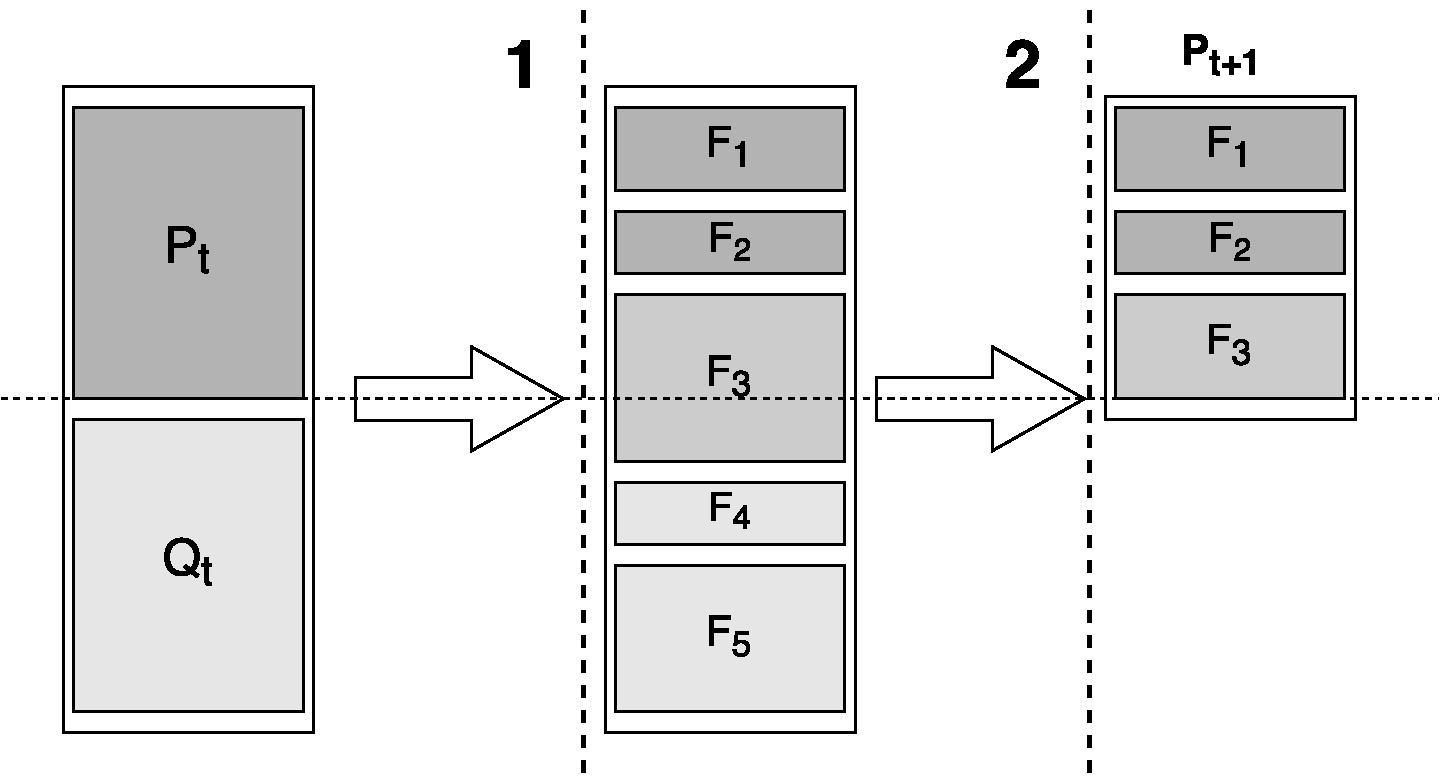
\includegraphics[ clip, scale=0.5]{nsga2_fronts}}
	\centering
	\caption{Uproszczony schemat działania algorytmu NSGA-II.\\1.Sortowanie rozwiązań niezdominowanych.\\2.Sortowanie w oparciu o lokalna wartość zagęszczenia.}
	\label{fig:nsga2_fronts}
\end{figure}

Na nowej populacji $P_{t+1}$ stosowany jest następnie zmodyfikowany operator selekcji. Użycie takie operatora zakłada, że każdy osobnik charakteryzuje się dwoma cechami:\\
\begin{enumerate}
	\item Numerem frontu, na którym się znajduje.
	\item Lokalną wartością zagęszczenia, która opisana zostanie później.\\
\end{enumerate}
Bazując na tych dwóch cechach, osobnik $i$ jest lepszy od osobnika $j$, jeśli:\\
\begin{enumerate}
	\item Osobnik $i$ znajduje się na lepszym froncie niż osobnik. $j$
	\item Osobnik $i$ znajduje się na tym samym froncie co osobnik $j$ ale charakteryzuje się mniejszą lokalną wartością zagęszczenia.\\
\end{enumerate}
Pierwszy warunek jest odzwierciedleniem konceptu dominacji. Osobnik leżący na lepszym froncie dominuje osobnika znajdującego się na froncie gorszym. Drugi warunek został wprowadzony, aby rozstrzygać, który z osobników jest bardziej wartościowy jeśli oba leżą na tym samym froncie. Jak zostało wyjaśnione wcześniej rozwiązując wielokryterialne problemy optymalizacyjne należy skupić się nie tylko na jakości rozwiązań ale również ich różnorodności. Różnorodność danego rozwiązania na tle całości populacji jest definiowana za pomocą metryki określającej zagęszczenie opisanej w \ref{blah}. 

Polega ona na obliczeniu średniego dystansu pomiędzy dwoma najbliższymi sąsiadami danego osobnika, znajdującymi się po jego przeciwnych stronach. Zostało to zilustrowane na rysunku \eqref{fig:nsga2_cd}. Takie obliczenia są przeprowadzane $m$ razy dla każdego osobnika, gdzie $m$ jest liczbą zdefiniowanych kryteriów. Następnie wyniki otrzymane dla każdego kryterium są agregowane do jednej wartości $d_{i}$. Generalnie algorytm obliczający zagęszczenie populacji można przedstawić następująco:\\
\begin{enumerate}
	\item Dla każdego osobnika z populacji przypisz $d_{i} = 0$ oraz zdefiniuj $l$ jako liczbę osobników.
	\item Dla każdego kryterium $m$, posortuj populację względem wartości funkcji oceny danego kryterium $f_{m}$, tworząc wektor $I^{m}$
	\item Pierwszemu i ostatniemu osobnikowi z wektora $I^{m}$ przypisz dużą wartość zagęszczenia: $d_{I^{m}_{1}} = d_{I^{m}_{l}} = \infty$. Reszcie osobników przypisz wartość zagęszczenia korzystając ze wzoru:
	\begin{equation}\label{eq:dist_eq}
		d_{I^{m}_{j}} = d_{I^{m}_{j}} + \dfrac{f_{m}^{(I^{m}_{j+1})} - f_{m}^{(I^{m}_{j-1})}}{f^{max}_{m} - f^{min}_{m}}
	\end{equation}
\end{enumerate}
$I_{j}$ oznacza osobnika znajdującego się na $j$-ej pozycji w posortowanym wektorze $I^{m}$. Wynika z tego, że $I_{1}$ oraz $I_{l}$ są osobnikami charakteryzującymi się kolejno najgorszą oraz najlepszą wartością funkcji oceny w porównaniu do całości populacji. Prawa strona równania \eqref{eq:dist_eq} jest różnicą wartości funkcji oceny dwóch najbliższych sąsiadów osobnika $I_{j}$. Jak łatwo zauważyć różnica ta jest połową obwodu prostokąta przedstawionego na rysunku \eqref{fig:nsga2_cd}. Dodatkowo wyliczony dystans jest dzielony przez różnicę pomiędzy największą ($f^{max}_{m}$), a najmniejszą ($f^{min}_{m}$) wartością przyjmowaną przez funkcję oceny $f_{m}$. 
\begin{figure}[!htb]
	\makebox[\textwidth]{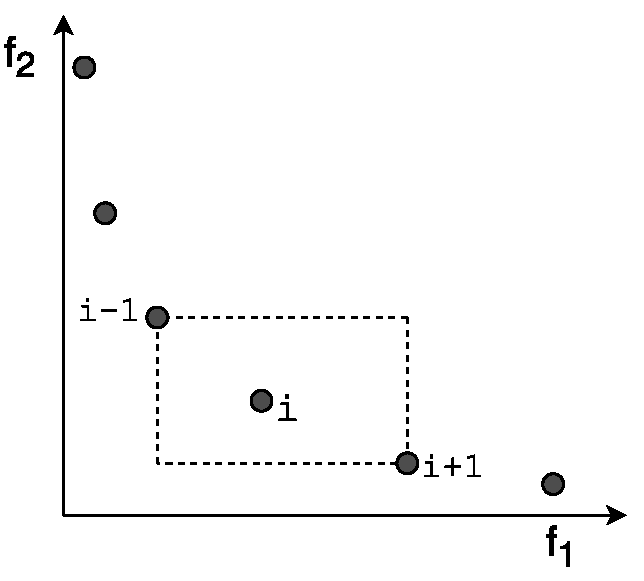
\includegraphics[ clip, scale=0.5]{nsga_2_cd}}
	\centering
	\caption{Reprezentacja najbliższego sąsiedztwa punktu $i$}
	\label{fig:nsga2_cd}
\end{figure}
\\Podsumowując schemat działania algorytmu NSGA-II wygląda następująco:\\
\begin{enumerate}
	\item Połącz populację rodziców $P_{t}$ z populacją potomków $Q_{t}$ tworząc grupę $R_{t}$.
	\item Na $R_{t}$ zastosuj sortowanie rozwiązań niezdominowanych w celu zdefiniowania frontów rozwiązań.
	\item Utwórz nową populację $P_{t+1}$ za pomocą opisanej wcześniej procedury.
	\item Utwórz nową populację potomków $Q_{t+1}$ za pomocą zmodyfikowanego operatora selekcji oraz standardowych operatorów krzyżowania oraz mutacji.\\
\end{enumerate}

W opisanym powyżej algorytmie NSGA-II różnorodność znalezionych rozwiązań niezdominowanych jest zapewniona poprzez zastosowanie zmodyfikowanego operatora selekcji. Osobniki rywalizują ze sobą opierając swoją wartość o front, na którym się znajdują oraz lokalną wartość zagęszczenia. Wartość zagęszczenie staje się szczególnie ważna w późniejszych momentach symulacji, kiedy większość osobników znajduje się już na najlepszym froncie. Biorąc pod uwagę fakt, że algorytm operuje na grupie o rozmiarze $2N$ istnieje duża szansa, że liczba osobników z pierwszego frontu jest większa niż $N$, a więc w celu wybrania najlepszych osobników wzięta zostanie pod uwagę wartość zagęszczenia. W konsekwencji rezultatem będzie zbiór rozwiązań niezdominowanych, cechujący się wysokim stopniem różnorodności.
\subsection{SPEA}
SPEA (Strength Pareto Evolutionary Algorithm) jest algorytmem zaproponowanym w 1998 roku. Koncept elitaryzmu jest tutaj wprowadzony w postaci zewnętrznej populacji $\overline{P}$. W populacji tej przechowywane są wszystkie niezdominowane rozwiązania znalezione w trakcie działania algorytmu. SPEA oprócz przechowywania najlepszych rozwiązań wykorzystuje je także w procesie reprodukcji, co ma znaczący wpływ na jakość generowanych potomków.

Pierwszym krokiem algorytmu jest utworzenie losowej populacji $P_{0}$ oraz pustej zewnętrznej populacji $\overline{P_{0}}$ o ustalonym rozmiarze, nie większym niż $N$, gdzie $N$ jest wielkością populacji $P_{0}$. Na początku każdej iteracji $t$, na populacji $P_{t}$ stosowane jest sortowanie rozwiązań niezdominowanych, w celu znalezienia najlepszego frontu. Osobniki znajdujące się na tym froncie są dodawane do populacji zewnętrznej. Następnie z populacji zewnętrznej usuwane są osobniki zdominowane przez nowo dodane rozwiązania. W ten sposób w populacji zewnętrznej zawsze będą znajdować się jedynie osobniki najlepsze. Łatwo uświadomić sobie, że wraz z działaniem algorytmu wielkość zewnętrznej populacji będzie rosnąć, aż do osiągnięcia zdefiniowanego wcześniej rozmiaru. Gdy ten zostanie osiągnięty pojawia się problem co robić z elitami znajdowanymi w kolejnych pokoleniach, skoro w populacji zewnętrznej nie ma już dla nich miejsca. Rozwiązaniem jest posłużenie jest wartością zagęszczenia, opisaną w poprzednim podrozdziale. Do populacji zewnętrznej trafiają osobniki charakteryzujące się największą różnorodnością na tle populacji. Jak zostało zasugerowane \ref{blah} wartość zagęszczenia może zostać zdefiniowana przy użyciu metryki wykorzystanej w algorytmie NSGA-II.

Kiedy populacja zewnętrzna zostanie zaktualizowana, następuje proces ewaluacji. Proces ten zostaje najpierw wykonany na populacji zewnętrznej. Dla każdego osobnika $i$ przypisywana zostaje wartość, zdefiniowana jako \textit{siła} $S_{i}$. Siła danego osobnika z zewnętrznej populacji wyrażona jest wzorem:
\begin{equation}\label{eq:str_ep}
	S_{i} = \dfrac{n_{i}}{N + 1}
\end{equation}
, gdzie $n_{i}$ określa liczbę osobników populacji, która jest zdominowana przez osobnika $i$. Jak łatwo zauważyć, osobnik dominujący więcej rozwiązań będzie charakteryzował się wyższą wartością funkcji $S_{i}$.\\\\
Osobniki z populacji $P_{i}$ ocenianie są przy użyciu następującej funkcji:
\begin{equation}\label{eq:str_p}
	F_{j} = 1 + \sum_{i \in \overline{P_{t}} \wedge i \preceq j} S_{i}
\end{equation}
Liczba $1$ zostaje dodana to po to, aby zapewnić, że wartość oceny każdego rozwiązania będzie większa od siły osobników znajdujących się w populacji zewnętrznej. Ponadto dodawana jest suma siły każdego osobnika, przez którego danego rozwiązanie $j$ jest słabo zdominowane. W tym miejscu warto zauważyć, że im mniejsza jest wartość funkcji oceny $F_{j}$, tym lepszy jest dany osobnik. Przykład procesu ewaluacji został przedstawiony na rysunku \eqref{fig:spea_eval}. Osobniki zaznaczone na czerwone należą do populacji zewnętrznej. Jak łatwo zauważyć w procesie reprodukcji faworyzowane będą osobniki charakteryzujące się mniejszą wartością funkcji oceny, a więc te z populacji zewnętrznej.
\begin{figure}[!htb]
	\makebox[\textwidth]{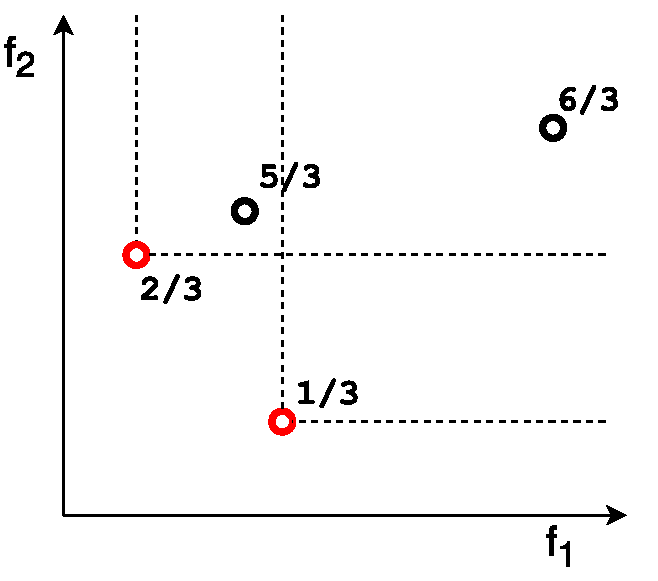
\includegraphics[ clip, scale=0.7]{spea_eval}}
	\centering
	\caption{Przypisanie wartości funkcji oceny}
	\label{fig:spea_eval}
\end{figure}

Po zakończeniu procesu ewaluacji, reszta procesu przebiega według standardowego schematu. Należy jednak pamiętać, że wszystkie operatory genetyczne działają zarówno na populacji $P_{t}$ jak i populacji zewnętrznej $\overline{P_{t}}$.\\\\
Podsumowując schemat działania algorytmu SPEA wygląda następująco:\\
\begin{enumerate}
	\item Zastosuj sortowanie niezdominowanych rozwiązań na populacji $P_{t}$ w celu znalezienia rozwiązań niezdominowanych.
	\item Skopiuj znalezione rozwiązania do populacji zewnętrznej $\overline{P_{t}}$.
	\item Z populacji zewnętrznej usuń rozwiązania zdominowane.
	\item Jeśli rozmiar populacji zewnętrznej jest większy niż $N$, zastosuj sortowanie w oparciu o wartość zagęszczenia oraz zredukuj rozmiar populacji zewnętrznej do $N$ pozbywając się najgorszych osobników.
	\item Oceń wszystkie rozwiązania korzystając z opisanych wzorów (\ref{eq:str_ep}, \ref{eq:str_p}).
	\item Utwórz nową populacje korzystając z operatorów selekcji, krzyżowania oraz mutacji.\\
\end{enumerate}

Analizując przedstawiony algorytm, łatwo zauważyć, że raz znalezione rozwiązanie optymalne w sensie Pareto nigdy nie przepadnie, ponieważ będzie przechowywane w populacji zewnętrznej. Jedynym sposobem na pozbycie się takiego rozwiązania jest znalezienie kolejnego rozwiązania optymalnego w sensie Pareto, lecz charakteryzującego się lepszą wartością zagęszczenia. Takie podejście zapewnia jakość oraz różnorodność znajdowanych osobników.

Duże znaczenie dla działania algorytmu ma wielkość zewnętrznej populacji $\overline{N}$. Jeśli ta jest duża (porównywalna do $N$)  nacisk na selekcję rozwiązań z populacji zewnętrznej będzie większy, co może prowadzić do tego, że algorytm nie będzie potrafił wygenerować rozwiązań leżących na prawdziwym froncie Pareto. Gdy $\overline{N}$ będzie zbyt małe, wpływ elitaryzmu będzie niezauważalny. Ponadto może to prowadzić do sytuacji w której wiele rozwiązań z populacji nie będzie zdominowanej przez żadnego osobnika z populacji zewnętrznej. Będzie skutkować to tym, że wartość funkcji oceny dla tych osobników będzie tak sama. Proponowaną wielkością populacji zewnętrznej jest $1/4$ wielkości populacji $N$.
\section{Strojenie}
Jak zostało opisane wcześniej działanie algorytmów genetycznych opiera się na wielu parametrach. Parametry te są ze sobą mocno  powiązane oraz znacząco wpływają na jakość symulacji. Proces wyboru odpowiednich wartości dla wspomnianych parametrów, nazywa się strojeniem.
\section{Implementacja}
W obu wybranych algorytmach (NSGA-II, SPEA) pojedynczy osobnik reprezentowany jest jako zbiór zraszaczy $S$. Maksymalna ilość zraszaczy została ustalona na poziomie $ms = 50$. Pojedynczy zraszacz jest reprezentowany jako następujący ciąg bitów:
\begin{figure}[!htb]
	\makebox[\textwidth]{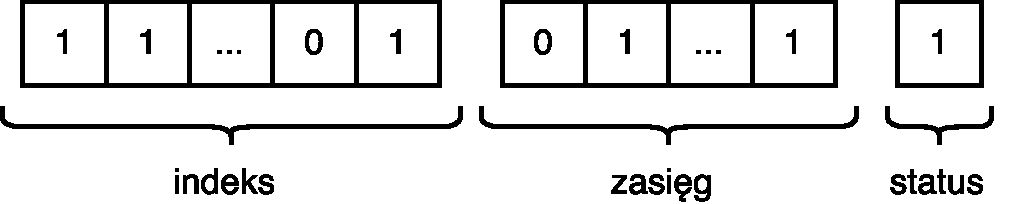
\includegraphics[ clip, scale=0.5]{sprinkler_bin_repr}}
	\centering
	\caption{Reprezentacja bitowa pojedynczego zraszacza}
	\label{fig:sprinkler_bin_repr}
\end{figure}
\\Ciąg binarny podzielony jest na trzy części. Pierwsza z nich odpowiada za indeks, czyli pozycję danego zraszacza. Zraszacz może znajdować się w jednym z kwadratów macierzy $M$, którego środek znajduje się w środku wielokąta $P$. Indeks danego kwadratu jest ustalany według wzoru:
\begin{equation}
	ind_{i} = n_{i} m + m_{i}
\end{equation}
, gdzie $n_{i}$ oznacza wierz macierzy $M$, w którym znajduję się kwadrat $i$; $m$ jest wartością wyrażającą szerokość macierzy; $m_{i}$ oznacza kolumnę macierzy $M$.\\\\
Długość części reprezentującej położenie danego zraszacza wynosi:
\DeclarePairedDelimiter{\ceil}{\lceil}{\rceil}
\begin{equation}
	L_{p} = \ceil[\big]{\log_{2} \text{ } ind_{p}} + 1
\end{equation}
, gdzie $ind_p$ jest liczbą reprezentującą największy indeks należący do $P$.

Kolejną częścią reprezentacji binarnej jest część odpowiadająca za zasięg danego zraszacza. Wymaga ona zużycia $L_{r}$ bitów, gdzie $L_{r}$ jest definiowane jako:
\begin{equation}
	L_{r} = \ceil[\big]{\log_{2} \text{ } r_{max}} + 1
\end{equation}
Wartość $r_{max}$ jest wartością oznaczającą maksymalny zasięg zraszacza. Jest ona definiowana na podstawie zbudowanej bazy danych i określana poprzez wybranie największej wartości zasięgu spośród wszystkich dostępnych.

Ostatnia, trzecia część reprezentacji binarnej to jeden bit mówiący o statusie danego zraszacza. $b = 1$ oznacza, że dany zraszacza został wybrany do rozwiązania oraz będzie uwzględniany w obliczeniach. W przeciwnym wypadku $b = 0$.\\\\
Podsumowując długość chromosomu każdego osobnika z populacji wynosi:
\begin{equation}
	L = ms(L_{p} + L_{r} + 1)
\end{equation}
W tym miejscu warto zauważyć, że długość chromosomu jest zawsze stała. Nieaktywne zraszacze ($b=0$) nie są w żaden sposób usuwane z reprezentacji. Takie podejście niweluje problemy pojawiające się przy użyciu reprezentacji chromosomów o zmiennej długości. Problemy te są najczęściej powiązane z trudnościami w implementacji operatorów krzyżowania oraz selekcji.

Oba algorytmy zaimplementowane zostały z wykorzystaniem selekcji turniejowej o rozmiarze turnieju równym 2, krzyżowania dwupunktowego (z losowym wyborem punktów podziału) oraz mutacji binarnej. Wskutek przeprowadzonego procesu strojenia ustalono, że algorytmy najlepiej pracują na następującym zestawie parametrów:\\
\begin{itemize}
	\item Prawdopodobieństwo krzyżowania : $0.9$.
	\item Prawdopodobieństwo mutacji : $0.05$.
	\item Wielkość populacji zewnętrznej (SPEA) : $1/4$N.
\end{itemize}

\chapter{Systemy wspomagania decyzji}

\chapter{Rozwiązanie problemu}
\section{System wspomagania decyzji}
\subsection{Architektura}
\subsection{Interakcja z użytkownikiem}
\section{Optymalizacja}

\subsection{Porównanie algorytmów genetycznych}
\subsubsection{Plan badań}
Złożoność oceny algorytmów służących do optymalizacji wielokryterialnej jest znacznie większa niż tej dla algorytmów rozwiązujących problemy obejmujące jedno kryterium. Wynika tak z samej definicji rozwiązania problemu wielokryterialnego, która wyjaśniona została wcześniej. Oceniając rozwiązanie takiego problemu należy wziąć pod uwagę następujące składowe:
\begin{itemize}
	\item Dystans znalezionego niezdominowanego zbioru rozwiązań od prawdziwego zbioru Pareto
	\item Równomierny rozkład znalezionych rozwiązań
	\item Długość przedziału pokrytego przez znalezione rozwiązania
	\item Czas wykonania algorytmu\\
\end{itemize}
Na potrzeby analizy i oceny dwóch zaproponowanych algorytmów wybrane zostały cztery metryki:
\begin{enumerate}
	\item \textit{Współczynnik błędu (ER):} wskazuje procent rozwiązań, które nie należą do prawdziwego zbioru Pareto.
	\begin{equation}
		ER = \dfrac{\sum_{i=1}^{n} e_{i}}{n}
	\end{equation}
	Gdzie $n$ jest liczbą znalezionych niezdominowanych rozwiązań; $e_{i}$ zmienną określającą czy dane rozwiązanie znajduje się w prawdziwym zbiorze Pareto. Jeśli $e_{i} = 0$ rozwiązanie znajduje się w prawdziwym zbiorze Pareto, w przeciwnym razie $e_{i} = 1$. $ER = 0$ oznacza idealne rozwiązanie.\\
	\item \textit{Równomierny rozkład (SP):} metoda mierząca wariancję dystansu sąsiadujących rozwiązań znajdujących się na znalezionym froncie Pareto.
	\begin{equation}
		SP = \sqrt{\dfrac{1}{n-1}\sum_{i=1}^{n}{(\overline{d} - d_{i})}^{2}}
	\end{equation}
	Gdzie $n$ jest liczbą znalezionych niezdominowanych rozwiązań; $d_{i}$ oznacza dystans Euklidesowy pomiędzy danym rozwiązaniem, a jego najbliższym sąsiadem; $\overline{d}$ jest wartością oznaczającą średni dystans pomiędzy rozwiązaniami. Wartość $SP = 0$ oznacza, że znalezione rozwiązania są rozłożone równomiernie.\\
	\item \textit{Jakość ogólna (DG):}  wskazuje jak daleko od prawdziwego zbioru Pareto znajduje się zbiór znalezionych niezdominowanych rozwiązań. Miara zdefiniowana w następujący sposób:
	\begin{equation}
		DG = \dfrac{\sqrt{\sum_{i=1}^{n} d_{i}^{2}}}{n}
	\end{equation}
	Gdzie $n$ oznacza liczbę znalezionych niezdominowanych rozwiązań; $d_{i}$ jest dystansem Euklidesowym pomiędzy danym rozwiązaniem, a najbliższym rozwiązaniem należącym do prawdziwego frontu Pareto. Wartość $DG = 0$ oznacza, że wszystkie znalezione rozwiązania leżą na prawdziwym froncie Pareto.\\
	\item \textit{Długość frontu (FE):} metoda wskazująca jak duży obszar jest pokryty przez znalezione niezdominowane rozwiązania.
	\begin{equation}
		FE = \sum_{k=1}^{K} \max_{i, j!=i} \sqrt{(f_{i}^{k} - f_{j}^{k})^{2}}
	\end{equation}
	Gdzie $K$ oznacza liczbę funkcji celu; $f_{i}^{k}$ jest wartością $i$-tego rozwiązania z perspektywy kryterium $k$.\\
\end{enumerate}
Aby skorzystać z powyższych metryk konieczne jest znalezienie prawdziwego frontu Pareto. Na potrzeby badań został on wygenerowany   poprzez wybranie niezdominowanych rozwiązań ze skumulowanej puli rozwiązań powstałej na skutek uruchomienia symulacji 10 razy dla każdego algorytmu. Rezultaty każdej symulacji były dodawane do puli po czym zredukowane do rozwiązań niezdominowanych.\\
Dla badań przygotowanych zostało 6 przypadków testowych. Zostały one podzielone ze względu na wielkość obszaru mającego zostać nawodniony oraz tego czy algorytm ma minimalizować nawadnianie poza zaznaczonym obszarem. Kształt wybranych obszarów został dobrany tak, aby jak najlepiej wizualizować wpływ ograniczeń na działanie algorytmów.

\begin{table}[]
\centering
\caption{Przypadki testowe}
\label{my-label}
\begin{tabular}{|l|l|}
\hline
Wielkość & Obszar \\ \hline
Mały & 1 \\ \hline
Średni & 2 \\ \hline
Duży & 3 \\ \hline
\end{tabular}
\end{table}

\subsubsection{Rezultaty badań}
\subsubsection{Podsumowanie badań}

\chapter{Podsumowanie}

\begin{mydef}
\textbf{Definicja} - pierwsza
\end{mydef}




 \clearpage
\appendix
\chapter{Appendix 1}


\clearpage
\pagestyle{plain}
\listofmyfigure
\listofmyequations
\listofmyalgorithm
\clearpage

%\bibliographystyle{apalike}%Used BibTeX style is unsrt

\bibliographystyle{iisthesis}
\bibliography{bibliography}

\end{document}

